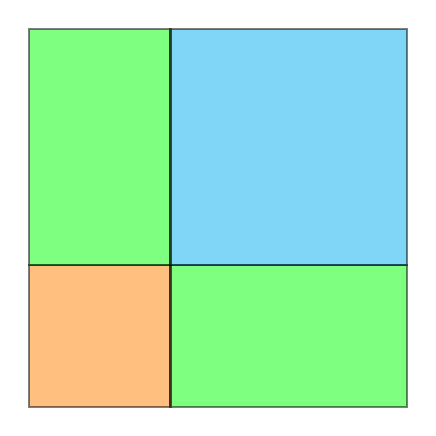
\begin{tikzpicture}[baseline=(current bounding box.north),scale=0.6]
    % cuadradito
    \draw[fill = orange, thick, opacity=0.5] (0,0) -- (3,0) -- (3,3) -- (0,3) --cycle;

    % ractangulos raices
    \draw[fill = green, thick, opacity=0.5] (3,0) -- (8,0) -- (8,3) -- (3,3) --cycle;
    \draw[fill = green, thick, opacity=0.5] (0,3) -- (0,8) -- (3,8) -- (3,3) --cycle;

    % Cuadrado 25

    \draw[fill = cyan, thick, opacity=0.5] (3,3) -- (8,3) -- (8,8) -- (3,8) --cycle;

\end{tikzpicture}